%% This is an example first chapter.  You should put chapter/appendix that you
%% write into a separate file, and add a line \include{yourfilename} to
%% main.tex, where `yourfilename.tex' is the name of the chapter/appendix file.
%% You can process specific files by typing their names in at the
%% \files=
%% prompt when you run the file main.tex through LaTeX.
\chapter{State of the Art}

In this chapter there will be an extensive explanation to the technologies used
throughout the document.



\section{Biometric factors}
%%[todo] add the description of the verious types of biometric authentications
Biometrics is the set of characteristics which allows a person to be identified
by one or more of its physiological traits. Biometric traits can be used for
authentication or identification of a person with a relatively high precision, and
usually are more secure than password or token based authentications. Some examples
of biometric factors typically used in authentication are: DNA, retina, iris, palm
veins, fingerprints and face recognition. There is another subclass of biometric
factors also called behavioral patterns, which relates more to the behavior of a person
like typing, gait and voice.\\
Due to its nature biometric factors depends on the technology used to gather them,
introducing some noise or errors, for which exists some metrics to evaluate their
reliability:

\begin{itemize}
    \item \textbf{False match rate} related to the probability of the system to
    match incorrectly pattern an input to a non-matching element in the database.
    \item \textbf{False non-match rate} is the probability that the system will reject
    a correct input.
    \item \textbf{Equal error rate}, the rate at which acceptance and rejection error is
    equal. The lower the better.
    \item \textbf{Failure to enroll rate}, rate at which the system fails to create
    a pattern from an input, typical of low quality inputs.
    \item \textbf{False to capture rate}, rate at which the systems fails to detect
    a biometric input.
\end{itemize}
\subsection{Speaker recognition}
Identifying a person by his or her voice is an important trait taken for granted
in human to human interaction.\cite{speaker-recognition} Everyday we use the voice as an identification pattern
to distinguish people we are not seeing, to remember people
we've met a long time ago whom face we are not recognizing.
Moreover humans ability to identify a person by the voice grows linearly
with the familiarity with the person they're talking with, arriving at the point
of recognizing someone just from their laugh. On the other hand it is
also true that we as humans find sometimes hard to remember a one-time heard voice,
or having a tough time recognizing someone from the phone.\\
Speaker recognition can be accomplished in three ways:
\begin{description}
    \item[Naive speaker recognition] is the process of recognizing familiar
    voices without any conscious training. This process is used daily by most of the people
    when interacting to each other.
    \item[Forensic speaker recognition] is the process used by forensics to identify
    criminals from their vocal activity. Special listeners are trained to listen phone
    conversations activity from suspects and compared with the criminal records, trying
    to find any match between them.
    \item[Automatic speaker recognition] is the process used by computers to learn
    about a human and then recognize known voices in audio files.
\end{description}

Speaker recognition is a large topic of research which includes two separated taks: speaker
identification, speaker verification and speaker diarization. Although we will focus mainly on the identification,
speaker verification happens when an unknown claims to be a known person and the task
of the system is to verify the correctness of the claim.
In speaker identification the task is to identify an unknown speaker from a set of known speakers,
using audio samples to find the closest speaker to him or her.
Finally, speaker diarization is the process of partitioning an audio stream in clusters relatively
to the different speakers in the recording. It is usually combined with speaker recognition and it answers
the question: \textit{Who spoke when?}.
We define \textit{closed} or \textit{in-set scenario}
when all the speakers are known and \textit{out-of-set speaker identification} when the potential input
may be out of the predefined speaker group.
Moreover speaker recognition can be:
\begin{description}
        \item[Text dependent] when the content of the speech is important to the
        identification of the person. Different people have different patterns of
        using words, adding a new trait of distinction between humans. This is usually
        used to authenticate users in restricted systems or resources.
        \item[Text independent] when the content doesn't influence the recognition
        of a known speaker but only the voice traits are used to identify the person.
\end{description}
Human speech is a performance biometric, making it intrinsic different from the majority
of the common biometrics (e.g. iris, fingerprints, footprint etc). This is due to the
identification made on how something is said rather than what, with a larger
degree variability. As can be seen in figure \ref{fig:sourcesvar} The sources of variability in speaker recognition can be partitioned
in three major classes: speaker based, conversation based and technology based.

\begin{figure}[h]
\caption{Sources of variability in speaker recognition}
\label{fig:sourcesvar}
\centering
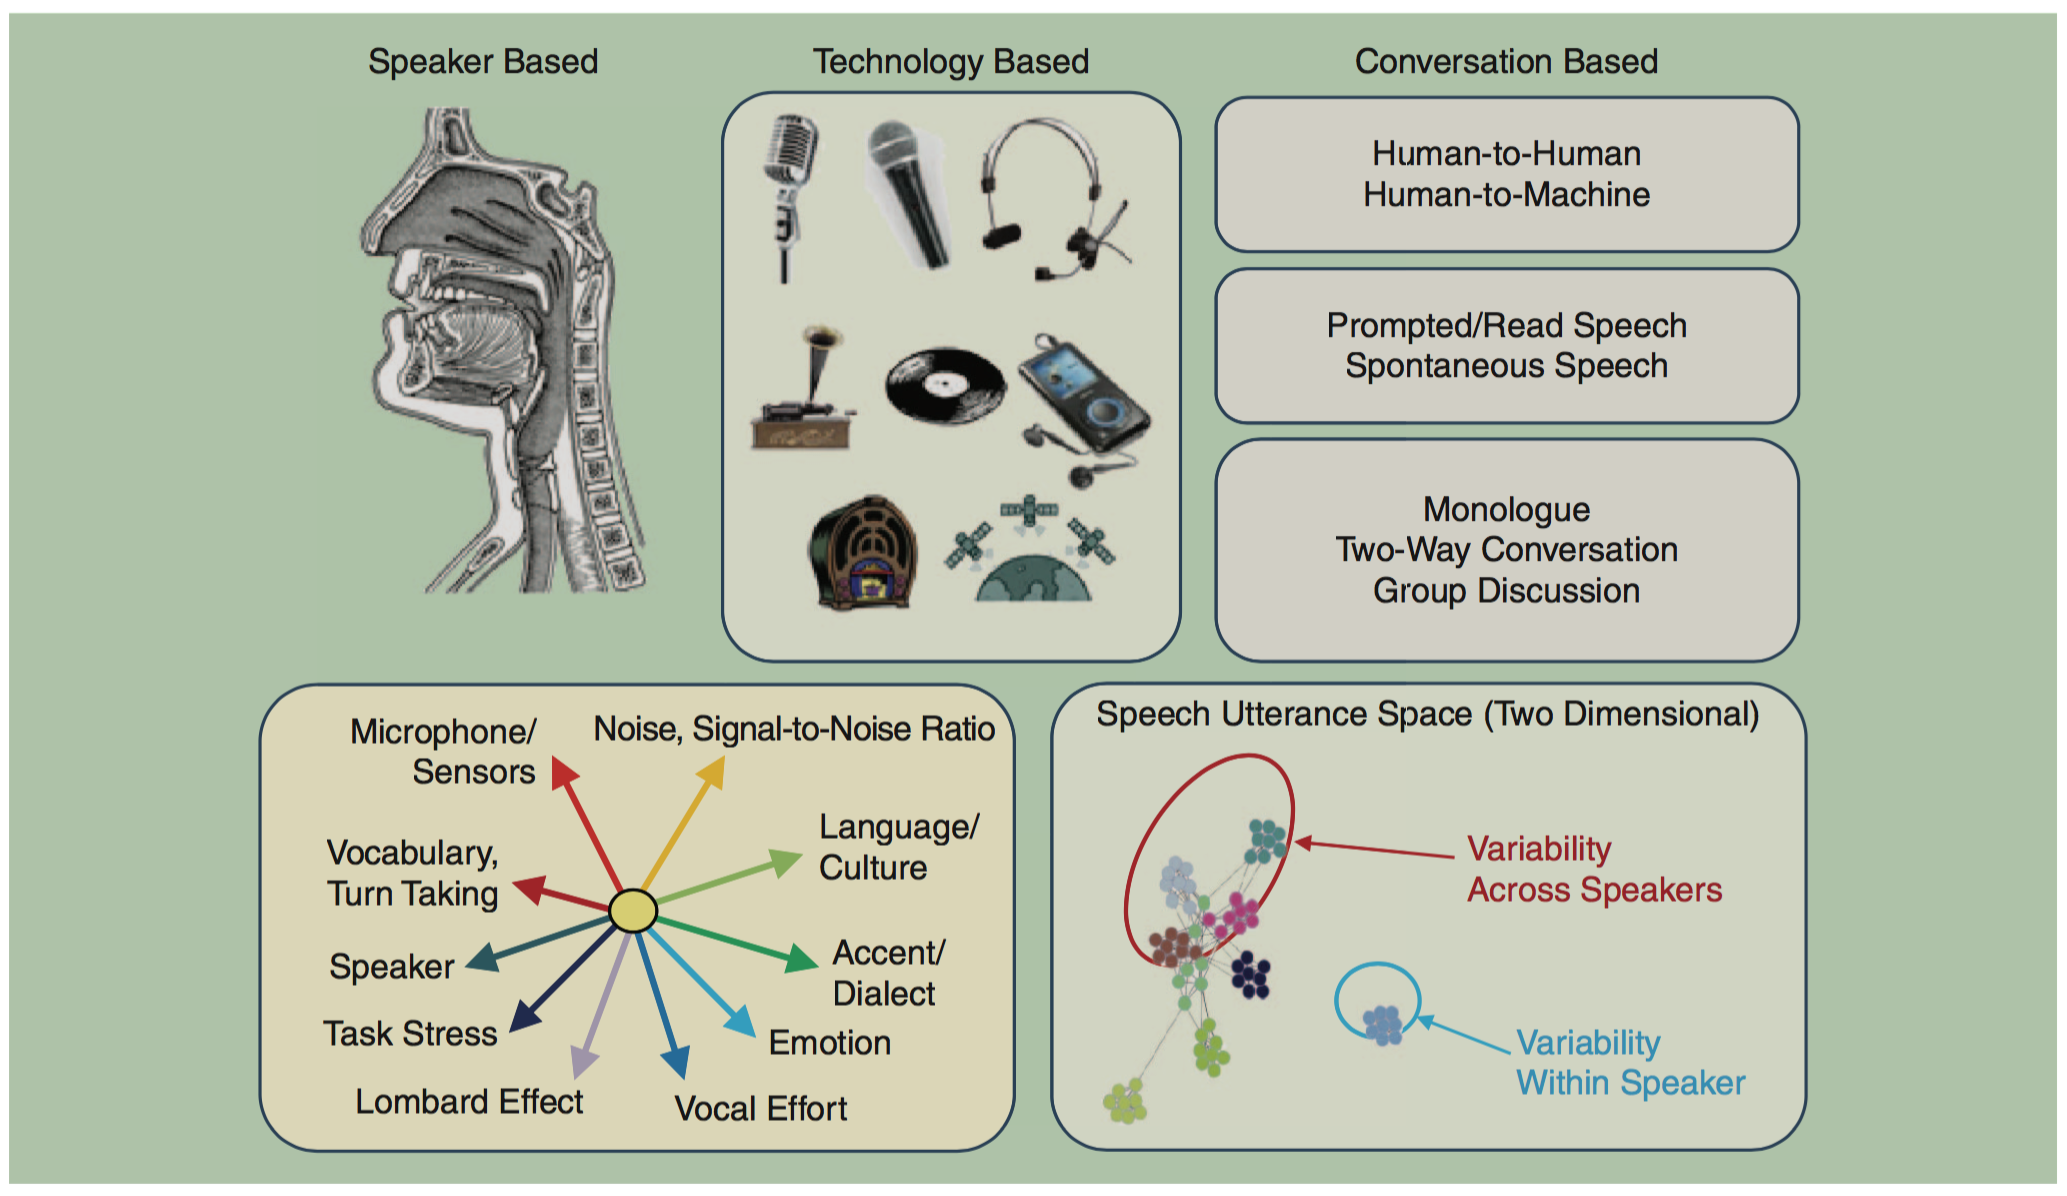
\includegraphics[scale=0.20]{sourcesvariability.png}
\par{Source: Speaker Recognition by Machines and Humans}

\end{figure}

\subsubsection{Speaker based variability}
These sources of variability depends on the speaker voice traits,
for which a range of changes of how the speaker produces a speech and
include the following factors:

\begin{description}
    \item[Situational task stress] when the speech is influenced by a task,
    typically stressful, made by the speaker. This usually happens when someone
    is speaking meanwhile doing some task such as driving, calling for an emergency.
    All these tasks includes cognitive or physical stress which introduces variability
    in how the speaker speaks.
    \item[Vocal effort/style] happens when the speaker alters his or her voice to react to
    a noisy situation modulating his or her voice to the situation; furthermore this happens
    also when singing.
    \item[Emotion] introduces a bias while speaking due to the human instinct of communicating
    the speaker emotional state through the tone of his voice.
    \item[Physiological] source is related to the physiological state of the speaker which
    can alter the normal voice trait for situations including: illness, cold, aging or medications / surgery.
    \item[Disguise] is a variability introduced by an intentional alteration of the speaker's voice
    for exceptional circumstances such as mimicking someone or avoiding detection.
\end{description}



\subsubsection{Conversation based variability}

These sources of variability are reflected from the conversational
situation of the speaker, including the interaction with a human
or with a machine.

\begin{description}
    \item[Human-to-Human] speech which may include two or more
    people interacting and discussing as well as one person addressing
    an audience. It may also consider different cases involving remote conversation
    through computer with headphones and a monologue.
    \item[Human-to-Machine] speech involving an interaction between a human
    speaker and a machine. This is mostly the case when a human has to adapt his
    voice to be understood by a computer, for example when using a virtual assistant, namely
    Siri.
\end{description}


\subsubsection{Technology based variability}
These sources are introduced by the technology used to acquire
the speech, mostly depends on the quality of the input (microphones).
Noise is typically introduced from the following channels:

\begin{itemize}
    \item electromechanical - which includes the
    transmission channel used to acquire the input.
    \item environmental - all the noises introduced by the background or from
    outside all the input components. Some examples may be white noise, background noise
    from the sun or the environment.
    \item data quality—duration, sampling rate, recording quality, and audio codec/compression.
\end{itemize}

\subsubsection{Feature Parameters}
Each speaker voice has some insight characteristics which identifies uniquely
the voice. Individual traits taken from the speaker vocal tract physiology or
from the articulation learnt during the time (i.e. dialects).
These traits are also called \textit{feature parameters}, defined as a set
of measurable and predefined aspects of a speech to be considered for a meaningful
comparison between two different voices. Typically multiple features
are used to identify a voice, and is more important if we consider the noise introduced by
the previous sources, which makes having many features an important aspect to consider.
Different voices may have similar or identical values for a specific feature but differ in all
the others.
As outlined from Nolan \cite{phonetic}, typical features has to have the following properties:
\begin{itemize}
    \item High between-speaker variability and low within-speaker variability
    \item Resistance to disguise and mimicry
    \item Robust in transmissions
    \item High frequency of occurrence in materials
    \item Easy to extract and measure

\end{itemize}

\subsection{Speaker Recognition algorithms}

In the following sections we'll provide a brief introduction
to the state-of-the-art of speaker recognition methods.

\subsubsection{Gaussian Mixture Model Based}

A Gaussian Mixture Model (GMM) is a combination of probability
density functions (PDFs) used to model multi-variate data\cite{speaker-recognition}.
GMM will provide a score evaluating the PDFs at different times, which
will be used to calculate the similarity between a speaker's GMM and an
unknown speaker. During an identification the system will calculate
a GMM for each known speaker, and use it to make comparisons between
for which the highest ranking will be selected.\\
Before GMM there were Vector Quantization(VQ) methods, which used
sets of prototypes instead of PDFs to build models for the speakers.
However GMM proved to be better because of its probabilistic model being
able to relate better to data despite of the more restrictive VQ model.
The Model is represented by the sum of the individual PDFs, where a random
vector $x_{n}$ can be modeled by $N$ gaussians with mean vectors $\mu_{g}$ and
covariance matrices $\Sigma_{g}$, where g=1,2...$N$. The PDFs $x_{n}$ is given by

\begin{equation}
    f(x_{n}|\lambda) = {\sum_{g=1}^N \pi_{g}N(x_{n}| \mu_{g}, \Sigma_{g})}
\end{equation}

where $\pi_{g}$ is the weight related to the $g_{th}$ component. The model
is denoted by $\lambda = \{ \pi_{g}, \mu_{g},\Sigma_{g}| g=1...N\}$, where the
probability of a feature vector given the GMM can be calculated with the above equation.
Given a GMM the probability of observing a sequence of feature vectors $X=\{x_{n}| n \in 1..T\}$
can be computed as

\begin{equation}
    p(X | \lambda) = {\prod_{n=1}^Tp(x_{n}| \lambda)}
\end{equation}


\subsubsection{GMM-UBM Speaker Verification}

Although GMM model based techniques are effective for speaker
identification tasks, to achieve speaker recognition a further
speaker model is needed. The new approach implies the use of
a \textit{Universal Background Model} (UBM) as alternate speaker model.
The idea behind UBM is to represent everyone except the speaker itself, essentially
a large GMM trained to represent the generic speaker-independent distribution
of speech features.\\
GMM-UBM is an approach combining the previous GMM model adapting it from
the UBM using Bayesian adaptation. The model is obtained updating a well
trained UBM instead of calculating the maximum likelihood training of the GMM
for a speaker. Speaker models obtained from the adaption of a trained UBM
are more reliable than GMM trained directly for each speaker.\cite{speaker-recognition}

\subsubsection{GMM Supervector SVM}

During the years research moved toward having fixed size representations
of speech. However this is far from reality where most of utterances used to train
models are of different duration lengths. A solution for the problem is the use of
\textit{supervectors}, a fixed size vector made concatenating all the variable duration
utterances parameters. A GMM supervector is typically obtained by concatenating
the GMM mean vectors of a MAP-adapted speaker model.\\
Supervectors can be used effectively using support vector machines (SVM) for speaker
recognition tasks. Basically the supervectors obtained from the training are used
as a positive example meanwhile different utterances are used as negative examples for
the model. An SVM classifier aim is to separate multidimensional data points obtained from two classes
on a hyperplane, and predict the class of an unknown observation from its location
on the hyperplane.
Given a set of training vectors and labels $(x_{n},y_{n}) for n \in \{1..T\}$ where
$x_{n} \in R^d$ and $y_{n} \in \{-1,+1\}$. Therefore an SVM goal is to learn
a function $f:R^d \rightarrow R$, for which the class label of an unknown vector x
can be predicted by:

\begin{equation}
    I(x)= sign(f(x))
\end{equation}

A hyperplane $H$ for linearly separable data given by $w^Tx+b = 0$ can be a class separator for
two classes as:

\begin{equation}
    y_{n}(w^Tx_{n}+b) \geq 1,n = 1...T
\end{equation}

The optimal situation happens when the  $H$ provides the maximum
margin between classes, the points ling on the margin are also known as support vectors.
An example of hyperplane can be seen in figure \ref{fig:gmmsvm}.
In conclusion this approach is considered very robust due to its ability
to combine the effectiveness of adapted GMMs with the discriminating ability of the SVM.
\begin{figure}[h]
\caption{Sources of variability in speaker recognition}
\label{fig:gmmsvm}
\centering
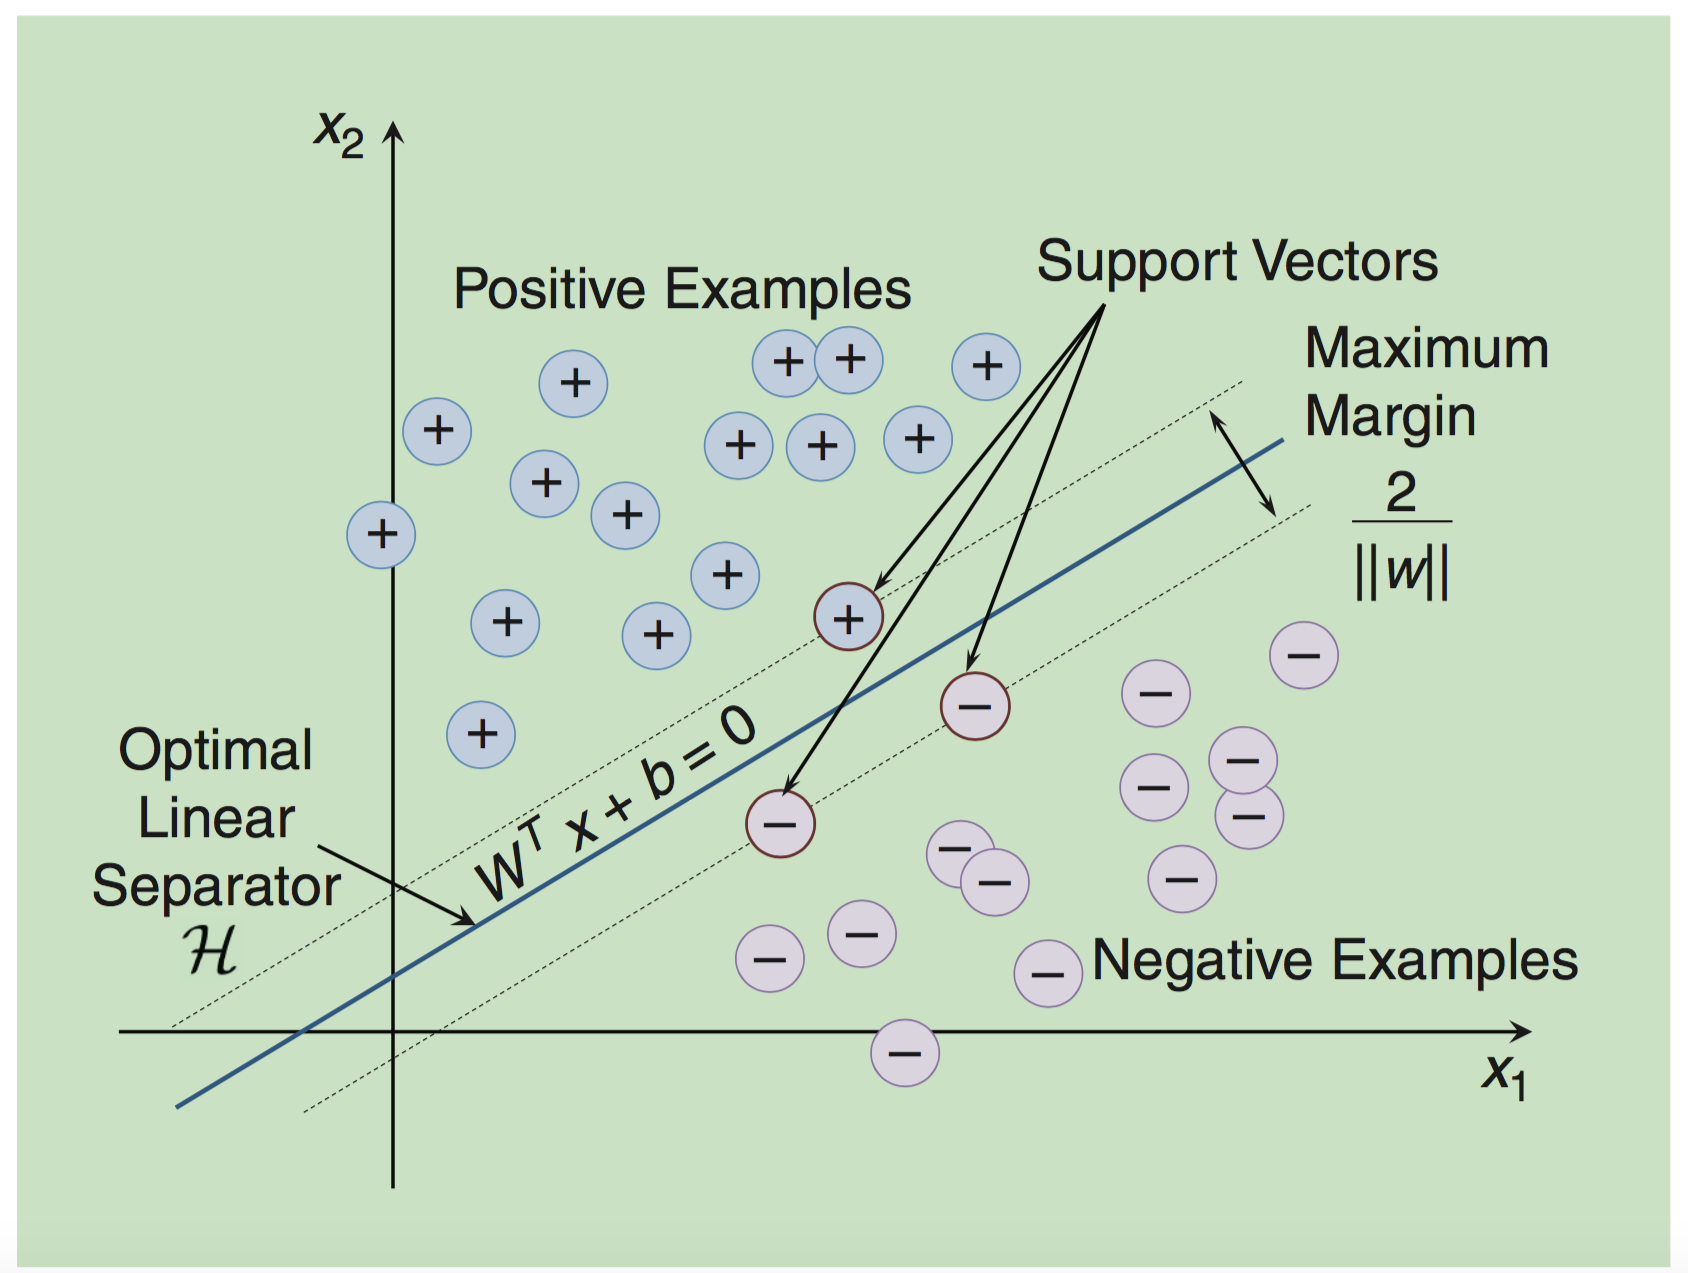
\includegraphics[scale=0.20]{gmmsvm.png}
\par{Source: Speaker Recognition by Machines and Humans}

\end{figure}



\subsubsection{Joint JFA}
The Joint Factor Analysis model is built combining both
eiganvoice and eiganchannel together, using a MAP adaptation
for a single model. The model basic assumption is that both
channel and speaker variability lies in the  lower dimensional
subspaces of GMMs supervector space. These subspaces are
modeled by two matrices $U$ and $V$, where for a random
utterance with speaker $s$ and session $h$ a GMM supervector
can represented by equation \ref{eq:gmmsv}
\begin{equation} \label{eq:gmmsv}
    m_{s,h} = m_{0} + Ux_{h} + Vy_{s} + Dz_{s,h}
\end{equation}
Joint FA exploits the behavior of speaker features in a variety of
conditions learned using FA \cite{speaker-recognition}.

\subsubsection{i-Vector Approach}

An i-Vector uses a set of low-dimensional factors(w) to represent the conversations
side. These factors controls an eigan-dimension of the total variability matrix (T) and
are also called \textit{i-vectors}.

\begin{equation}
    s = m + Tw
\end{equation}
Where
\begin{itemize}
    \item s is the conversation side supervector
    \item T the total variability matrix
    \item w is the i-vector
\end{itemize}
Unlike JFA or other factor analysis models, i-vector does not consider any
distinction between speaker and channel but rather consider them as a dimensional
reduction of a GMM supervector. I-Vectors effectively summarize utterances allowing
compensating methods that were unpractical before with large supervectors.

\section{Internet of Things}

\textit{Internet of Things}, better known as IoT, is the world of interconnected devices
connected to the real world and to the Internet. These devices has a very
broad definition, from the smart sensors in a power plant to the smart fridge in
a house. What connects these devices is their ability to be connected with the world,
sharing, with the needed restrictions, their work. This opened the door to a new
revolution in the IT sector, prompting new opportunities for developers, entrepreneurs
and end users. Some of the most relevant endings of these technologies are \textit{Smart Houses},
\textit{Smart Cities}, Cars etc. %[TODO] continue a little bit here

\subsection{Ecosystems}

An ecosystems is by definition \textit{a system, or a group of interconnected elements,
formed by the interaction of a community of organisms with their environment.},
in our case a set of smart devices connected between them. The IoT world is evolving
from distinct single entities to more evolved clusters of devices which can communicate
more easily between each other.These are usually are made by companies using specific protocols or standards
to simplify the connection between their products, but at the same time closing it to the others.
%[TODO] connect the two paragraphs
The list of products related to the \textit{Internet of Things} is too broad for
being even listed, due to the highly expanding sector related to smart devices.
However we will consider the most common ecosystems which can be easily found in a common
home, meaning services for: Smart Lights, Cameras, Thermostats etc. Luckily
most of them are being bought and integrated in bigger environments run by
famous companies such as \textit{Google} or \textit{Apple}.
The reason for which we try to restrict the integration with these ecosystems is
mainly practical, because they're the most common and they do offer simulators
for testing, and because they suits perfectly our scenario.

\subsubsection{Google - Nest}

\textbf{Nest}\cite{nest} is a home automation producer of smart devices
which ranges from their famous Smart Thermostat to the locking system, from the
washing machine to the light system, from the \textit{Dropcamera} to the Hi-Fi Sound system,and
these are just some examples. The number of components supported by this company
is wide, which makes it a good choice to support in our scenario, also because of
the high cost of these devices. The main added value given by these accessories is related
to two main points: saving money with a smart consumption of electricity and the ability
to remotely control the house with an easy to use application.
Besides the commercial value of \textit{Nest}, the platform offers many tools for developers
to interact with their platform using their Cloud service. Third party developers
are encouraged, with some limitations, to use their Cloud service which
offers some \textit{RESTful} APIs to gather access to the remote devices.
The remote access through APIs unlinks developers from platform dependent libraries (see later HomeKit)
that restricts the use or the integration with a specific technology.
Furthermore it is possible to access directly \textit{Nest} devices with their \textit{Nest Wave}
which allows direct communication with non-branded devices using two different communication protocols,
mainly \textit{802.11} standards.


\subsubsection{Apple - HomeKit}

\textbf{HomeKit}\cite{homekit} is a very similar ecosystem to the one described before, producing or supporting
home automation devices. \textit{HomeKit} relies on the large network of Apple devices,
making it an environment to be considered even if it is relatively new on the market. The key
point of \textit{HomeKit} is the easy integration with Apple devices, fitting almost perfectly wherever
there was an already existing Apple ecosystem. Developers are allowed to take control of the devices
only through iOS applications, restricting the possibilities of integration with different ecosystems or
technologies. Moreover it ties the developers to their technology making it really hard to be adopted in a different
system. However as we'll see later it is possible to bypass the problem using the microservice architecture to
make the system independent from specific technologies.


\subsubsection{Samsung - SmartThings}

\textbf{SmartThings}\cite{smart} is another ecosystem from \textit{Samsungs} with many similarities
with the former producers.\textit{SmartThings} focuses on four main Smart devices categories:
\textit{Security},\textit{Monitoring}, \textit{Lighting and Energy} and \textit{Convenience and Entertainment}.
\textit{SmartThings} as the previous ecosystem does not allow a direct interaction with the smart devices,
but offers a developer-friendly interface to their Cloud Service. However, as \textit{HomeKit} it is tied to
a technology, making it harder for different technology stacks to access.


\section{The Microservice Architectural Style}

\subsubsection{SOA vs Microservices}
In short, the \textit{microservice architectural style} is an approach to developing a single
application as a suite of small services, each running in its own process and communicating with
lightweight mechanisms, often an HTTP resource API. These services are built around business capabilities
and independently deployable by fully automated deployment machinery. There is
a bare minimum of centralized management of these services,
which may be written in different programming languages and use different data storage technologies.\cite{microarch}\\
There is a close link between the \textit{microservice architecture} and the \textit{service oriented architecture},
thus due to their nature the community classified microservices as a subclass of the service oriented architecture.
\textit{Don Box} of Microsoft described the Service-Oriented paradigm with the following four principles\cite{msdn}

\begin{enumerate}
  \item Boundaries are explicit
  \item Services are autonomous
  \item Services share schema and contracts, not class
  \item Service compatibility is based on policy
\end{enumerate}

Microservices fullfills the first two requirements, with a very strong focus on the second principle.
However the functionalities are very frequently exposed using a \textit{RESTful} interface, which
doesn't expose any contract nor schema. Furthermore microservices holds another subtle difference related to their
scope, where a microservice serves as a service inside its application meanwhile typical SOA services
serves a broader scope and \textit{can be} part of the same application.
The difference between the two concepts is very subtle, and it wouldn't be impossible for them
to be the same in certain situations. \textit{Bob Ruhbart} from Oracle described shortly the difference:
\textit{Microservices are the kind of SOA we have been talking about for the last decade. Microservices must be independently deployable,
whereas SOA services are often implemented in deployment monoliths.
Classic SOA is more platform driven, so microservices offer more choices
in all dimensions}\cite{microsoa}.

\begin{figure}[h]
\caption{Graphic illustration of microservices and SOA}
\centering
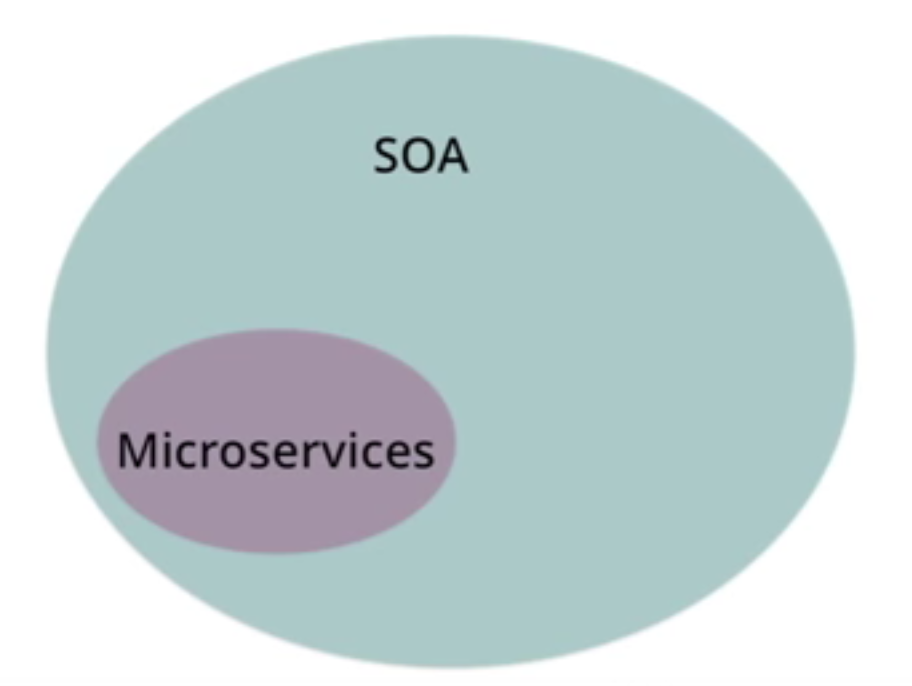
\includegraphics[scale=0.65]{soavsmicro.png}
\end{figure}

\subsection{Internal integration}
Typically when a new component has to be added to an existing
project the approach consists in the development of a library which
has the logic to deal with the new module to be supported. Subsequently the component
will
become part of the project itself, with its needs to be updated throughout time.
However when the number of components to integrate increases it will affect the size
of the project and very likely its performances.
In our case the component to be integrated will be the ecosystem driver,
having a set of libraries which are capable of interacting with the remote APIs or
with the direct wired connections. As we'll see in the next paragraph this is a typical
monolith approach, meanwhile for this situation would be better to use a microservice approach.

\subsection{Integration as a Service}
Considering the \textit{Microservice} architectural pattern we can decompose
the above situation creating dedicated services capable of handling the
required business logic to interact with an external system. This approach
is also called \textit{Componentization via Services}\cite{microarch}, where a component is defined
as a \textit{unit of software that is independently replaceable and upgradeable.}
It is important to distinguish between \textit{libraries} and \textit{services}:
the latter uses out-of-service components to communicate, mainly HTTP requests or
remote procedure calls when libraries uses instead mechanisms like in-memory calls.
The main advantage to build components as services instead of libraries is the
possibility to deploy them individually without the need to redeploy the whole system.
If a library is modified or removed the whole system will need to be redeployed,
which in most of the cases it is converted in a loss of money and time. That's not
the case if the system is composed by many independent systems, where only the changed
service will need a new deployment. However this is not always true, there will be some
circumstances where it will be necessary anyway to deploy again the whole system, but the
aim of this approach is to reduce the number of these necessities.

\subsection{Other benefits}
Apart from the benefits already listed formerly, there are other benefits introduced by
adopting the microservice architecture:

\begin{description}
  \item[Heterogeneity between technologies] Structuring the system as a set
  of services frees us from the limitations of a singular technology allowing
  us to adopt different frameworks for different tasks. This benefits on the
  possible optimization that can be achieved using the right technology for the
  right task. Furthermore this removes completely the problem of creating adapters
  for different technologies to integrate in the system if they do not exist. This is
  also called \textit{Decentralized Governance}.
  \item[Evolutionary Design] is a concept popularized by the \textit{Extreme Programming},
  where the system is continuously evolving during the phases of it's development.
  This key feature makes possible to evolve adopting a microservice architecture while
  keeping the old legacy monolith system, well tested and functional, without rewriting
  the whole system.
  \item[Designed for failure] Building a system made of services instead of components
  leads the developers to take more effort in considering failures. Developers have
  to take in consideration the possible failure while reaching the service, and
  prevent the system to crash and handle the situation in the most gentle way. On the
  other side, this approach introduces more overhead to handle the possible situations.


\end{description}


\subsection{Microservice Oriented Internet of Things}
IoT with their advent brought up some, not yet resolved, challenges which fits
very well with the Microservice architecture. \textit{Interoperability} is one of these
challenges aimed to be solved. Microservices \textit{decentralized governance} feature,
which allows the use of different technologies inside the same systems holds the key for
solving the interoperability problem. Key IoT devices vendors realizes that if their products
supports multiple interoperability standard they're likely to be adopted also by their
competitors (e.g. Nest products are available on HomeKit[?]). Microservices here can be
used as isolated adapters for the many different technologies, facing the spreading
fragmentation of communication protocols between machines.\\
Microservices are by nature dynamic and reactive, which makes them a good choice for
an environment where new technologies are frequently added or modified.

\section{Calvin}
  \textit{Calvin} is an Open-Source distributed framework designed mainly, but not only,
  for IoT systems. The key point of \textit{Calvin} is the "Distributed cloud for IoT", meaning
  running the code where it best suits the performance needs, a crucial aspect since we are
  dealing with low-resource components. We will use \textit{Calvin} for the whole course of the document,
  referring to it as the main "system", also used to integrate with the others. \\
  \textit{Calvin} has the ability to integrate new components without replacing them by writing
  proxies for the specific hardware to support. Proxies are actors written to handle
  communication with the legacy system. Such a proxy actor handles the task of converting data
  from the application into messages or requests the old system can handle, and converting the
  response back into tokens the Calvin application understands.\cite{calvin2}

        \begin{figure}[h]
        \caption{Proxies interaction}

        \label{fig:calvinproxy}
        \centering
        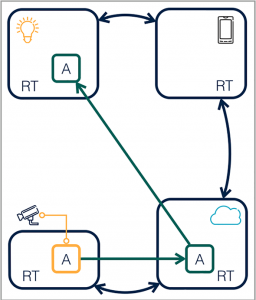
\includegraphics[scale=0.75]{calvin4.png}
        \par{Source: Ericsson Blog}
        \end{figure}
  Figure \ref{fig:calvinproxy} shows the interaction of native Actors and Actors which
  acts as a proxy for legacy components, in this example the camera.




  \textit{Calvin} is built upon the well-established actor model, using a methodology often referred to as dataflow programming \cite{calvin1}, and
  its life cycle can be summarized in four, well-distinct, phases: \textit{Describe}, \textit{Connect}, \textit{Manage}
  and \textit{Deploy}\cite{calvin-article}.

\subsection{Describe}
  The smallest functional units in \textit{Calvin} is an Actor. Actors do not share
  nor state or behavior, encapsulating all the logic. The key point of Actors in Calvin
  is their reactivity: they react to external events or when receiving inputs. Actors
  communicates only using data through ports, has to be defined before deploying the system.
  This way is possible to describe the possible interactions that the actor may have when
  connecting it to others.\\
  Having a non-shared internal state allow the Actor to be serialized and moved to another
  running machine or to be backed up if the machine crashes. However this is partly true because
  it may be tricky to serialize Actors with a very complex internal state.

  \begin{figure}[h]
  \caption{Describe Phase}

  \centering
  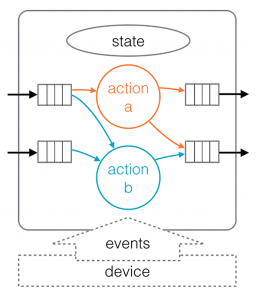
\includegraphics[scale=0.75]{calvin1.png}
  \par{Source: Ericsson Blog}
  \end{figure}


\subsection{Connect}

    \begin{figure}[h]
    \caption{CalvinScript Example}

    \label{fig:calvinscript}
    \centering
    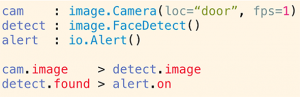
\includegraphics[scale=0.75]{calvin2.png}
    \par{Source: Ericsson Blog}
    \end{figure}

  After describing the many functionalities provided by the various Actors in the system
  we need to tie them to build applications. \textit{Calvin} offer a scripting language,
  named \textit{CalvinScript}, to describe the various connections between actors
  and their input and output ports. In figure \ref{fig:calvinscript} there is an example
  of a script for detecting faces in an image. The first part is relative to the actors declaration
  and initialization, giving a clear description of which actors will be playing in the current
  environment. The second part describes the links between each actors, structuring the flow
  of the process. In this case the actors in the system are 3: the \textit{Camera}, the \textit{Detector}
  and the \textit{Alert}. The flow of the process is relatively simple in this case, and it is structured
  as follows: the  \textit{Camera} takes a picture, which will be passed to the \textit{Detector}. Subsequently
  the \textit{Detector} will send its result to the \textit{Alert} actor, which will possibly fire an "alarm" if he
  detects any human face inside the picture.\\
  Figure \ref{fig:calvinactors} shows a more complex interaction between actors. %%[TODO] maybe add something here about the picture

  \begin{figure}[h]
  \caption{Actors interaction}

  \label{fig:calvinactors}
  \centering
  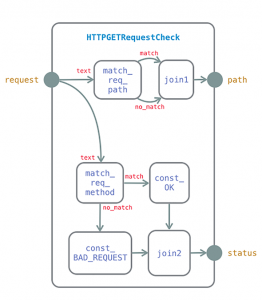
\includegraphics[scale=0.75]{calvin3.png}
  \par{Source: Ericsson Blog}
  \end{figure}



\subsection{Deploy}

  Each Actor has different resource requirements needs to be satisfied in order to be
  deployed successfully. For example, referring to the previous scenario, an actor
  using a camera needs to be deployed on a system where there actually is a camera. These
  are also called \textit{hard} or \textit{unconditional requirements}, which determines
  the possibility to instantiate or migrate the actor on a machine. \\
  On the other side there are also \textit{non-functional requirements}, describing where
  an actor would suit best for its task. Always referring to the former example, when applying
  face detection it would be better to perform this task on a more performing machine compared to
  a low-resource machine, like a \textit{Raspberry Pi}.\\
  However at the moment \textit{Calvin} supports only \textit{static deployment}, needing the user
  to define where to deploy and execute the actors.

\subsection{Manage}
  When the whole runtime is running it is more than needed to have a tool to keep
  track and monitor the activities in the system. The runtime can be queried to retrieve
  informations about the actors and locate them. It is also possible to track
  the actors firings, on which ports and step by step execution. These are mainly
  debugging tools, though it is also true that this is a recent framework and many
  functionalities are already in development.


\subsection{The relationship between the Actor Model and Microservices}
Actors are isolated, single-threaded components that encapsulates both state and behavior.
Typically actors communicates using lightweight direct messaging systems, for example
to receive or return inputs/parameters. Microservices are very similar to Actors in many
of their key aspects, such as isolation, encapsulation and lightweight messaging, though
usually microservices uses RESTful interfaces. There is some discussion
in the community whether some argues that actors are actually microservices
themselves \cite{microarch1} meanwhile others defines actors as a subset of microservices \cite{microactor}.
This however heavily depends on the actors framework adopted for the situation, which in our
case an Actor can not be compared to a microservice due to an insight limitation: \textit{Calvin Actors can not
use different technologies}, at the moment.

\subsection{Calvin's Three Tier architecture}

Calvin is structured with a three tier architecture: the actor layer, the system layer and the runtime layer.
Each of them is isolated and can communicate with each other only passing values through the various
layers. The architecture is summarized in picture \ref{fig:calvinlayers}

\begin{description}
    \item[Actor Layer] The actor layer is the upper layer which exposes all the actors and their functionalities.
    Actors can used only the functionalities offered by the lower level calvinsys with no direct access to the runtime
    system.
    \item[Calvinsys Layer] Calvinsys is considered the middleware, where all the runtime logic is exposed through
    high level functions and objects. This layers wraps and uses the functionalities offered by the runtime layer,
    offering tools for the development of advanced actors.
    \item[Runtime Layer] the runtime layer is considered the core, in this layer are stored all the low level
    implementation.In this layer can be found detailed implementations of how to communicate with different kinds
    of sensors, an asynchronous implementation of HTTP calls for Calvin and etc. Here's the core of all
    the functionalities adopted by the higher level objects such Actors or middleware libraries.
\end{description}

\begin{figure}[h]
\caption{Calvin Architecture}
\label{fig:calvinlayers}
\centering
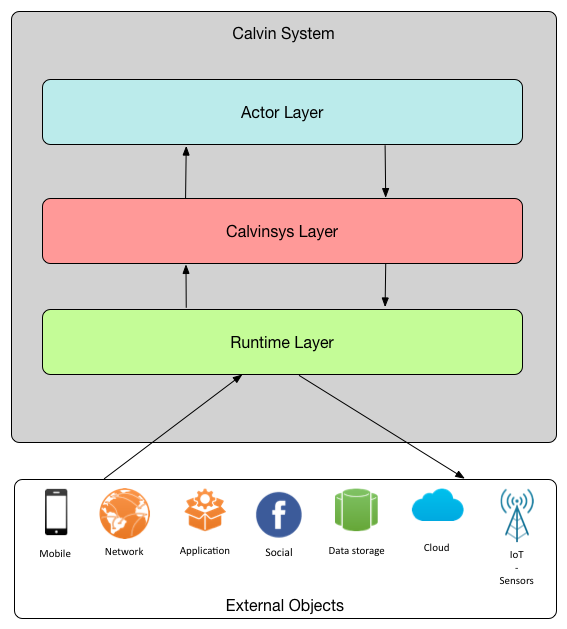
\includegraphics[scale=0.45]{calvinlayers.png}
\end{figure}


\subsection{Anatomy of an Actor}

As previously introduced Actors are abstract reactive entities which exposes inbound and outbound connections.
In contemplation of \textit{reactivity} all the actions taken from an actor must be simple, fast and short. Nonetheless
this optimal situation is hardly achievable in real life, it's usually more common to have blocking calls to services
in the runtime which require on average more then 1-2 seconds. This limitation can be solved simply moving the logic
in the runtime towards an asynchronous approach for long time tasks. Typical tasks requiring asynchronous interaction
can be reading data from a sensor, sending an HTTP request or authenticating into any service, the list is longer but
can summarize in most of interaction with out of the system objects.\newline
An actor anatomy can summarized in the following parts:
\begin{itemize}
    \item Declaration of the connections
    \item Initialization and setup
    \item Migration
    \item Actions, Guards and Conditions

\end{itemize}

\subsubsection{Declaring the connections}

All the connections of an actor has to be declared a priori, and hence be all used (or allocated)
when the actor is used. The declaration is done simply adding under a comment the names of the many connections
and their type: either input/output or both. Here is a simple example of an actor for HTTP GET requests:

\begin{verbatim}
    Input:
      URL : URL to get
      params : Optional parameters to request as a JSON dictionary
      header: JSON dictionary with headers to include in request
    Output:
      status: 200/404/...
      header: JSON dictionary of incoming headers
      data : body of request
\end{verbatim}

In this example we can see the 3 input ports: URL, params and header, which will all be needed to be set
in order to fire one of the actions, depending on the condition. These inputs can be used
as a condition parameter using \texttt{action\_input['var\_name']} and \texttt{action\_output['var\_name']}
for outputs.\\
However it is very likely that we won't need all these inputs or outputs, specially if they are optional
like \texttt{params}. For this reason there exists two special actors which will connect to these
ports without generating tokens or consuming them without doing anything (namely Void and Terminator).

\subsubsection{Initial phase}

The initial phase is denoted by the decorator \texttt{@manage['inputs']}, where all the variables
are set and the required libraries are loaded. It is possible to pass inputs at instantiation
time using manage and bypassing the input ports, though this approach is discouraged and
advised only for particular situations. Furthermore in this phase all the components
from the \textit{calvinsys} will be loaded for a consequent use during the actor actions.

\subsubsection{Migration}

One of \textit{Calvin's} key feature is the simplicity of migrating actors through the
different nodes in a cloud system. Migration of the object is achieved using a special function
\texttt{migrate(self):} to which can be passed the current actor object, and it will be serialized.
Migrating implies serializing all the current variables which composes the actor's state to be sent, though
problems may arise if these variable contains complex objects such as connections (e.g. DataBase connection,
TCP connection etc). When the state will be sent to another machine, this will setup the actor
passing from the former phase, hence creating a new (almost) identical actor.

\subsubsection{Actions, Guards and Conditions}

The core of an actor are the actions it can perform, but these needs some conditions to bet met
before being fired (e.g. having a variable set to \texttt{true}). Most of actions are composed of three
key elements:

\begin{description}
    \item[Condition] is a mandatory decorator which describes the inbound and outbound connections for the action.
    Although the name suggests it to be the condition statement to for firing an action, condition is related to the
    input and output condition of the action. An example of condition for a camera actor can be \\
    \texttt{@condition(action\_input=['trigger'], action\_output=['image'])}. In this case our actor when will receive a token
    on the \texttt{trigger} port will enable the action, but the next decorator will be the definitive check to pass to the action
    body.
    \item[Guard]  is an optional decorator, for checking some conditions before passing to the body of the action.
    Guard is more related to the internal state of the actor instead of the connected ports, thus it's the real condition
    check to fire the action. Guard can be used to see if a variable has been set or if its value is correct. For example
    if we want to check that an actor has completed an asynchronous task we can use a guard similar to this one:
    \texttt{@guard(lambda self: self.camera.picture\_taken)}. In this case \textit{Calvin} will perform an evaluation
    of one the actor internal objects: it the value is set to \texttt{true}, it means that the picture has been taken and
    its stream has been saved on the disk (i.e. the file exists). This allow the system to prevent firing actions
    when the actor may not be ready for it even though the firing connections are set.
    \item[Action] The action is a simple function which has to take as parameter the inbound values in the condition
    statement, and return an \texttt{ActionResult} object with the expected output bounded to the outbound values.

\end{description}

Moreover inside the actor the actions has to be listed by priority, to avoid ambiguity
when choosing with the correct action to fire.
